\chapter{Prologue: Learning from the Rise and Fall of the Ancient Maya}
\label{chapter:maya}

\section{Introduction}

% Geosimulations as one approach to understand geological realities.
Archeologists and historians try to understand archeological, geographical and geological records in terms of rulesets that explain the processes underlying the historical environmental conditions and societies that produced them.
Geosimulations are one way to implement and test such sets of rules by combining them with geographical and geological data, analyzing their results and inter-comparing them with the empirical findings. This strategy has proven useful especially for more complex sets of rules, where the impacts of changes in individual assumptions or parameters are difficult to track by logical reasoning alone. \textcolor{red}{[CITE SOME OF MAURITS WORK HERE]}

% the epistemological dimension of modelling
However, the design and calibration of such models heavily relies on empirical data, as well as reasonable assumptions about processes and storylines that can guide the analysis of the model. Based on these assumptions and the data at hand, a modeler usually defines the different parts of a model as agents that behave according to local rules that prescribe different actions for them depending on the current state of their environment and/or the actions of other agents. This raises the question, how the modeler can avoid to structure the agents in a model (in terms of equations, algorithmic rules and parametrization) to an extent that prevents the model from generating insights that go beyond the data, process models and storylines that went into the model construction in the first place.

From a conceptual perspective, the individual agent in such a model cannot show new (in the sense of autonomous) types of behavior anyway, since all its actions are fully determined by the prescribed set of rules. Even if these rules were involving some element of randomness, the modeller still had to specify this randomness with respect to its statistical properties. 

% agent-based models as a way out through emergent dynamical properties.
Yet, this does not mean that investigating the behavior of individual agents is not interesting. At the same time, many studies with agent-based models (ABMs) have illustrated, how at the system level various surprising effects can emerge from the interactions of many agents with individually well predictable behaviors \citep{Epstein1999}. \footnote{I use here a weak notion of emergence, which allows explaining macroscopic (global) phenomena on the basis of microscopic (local) interactions of the system's constituents that differ from the explained macro-phenomena. This is opposed to strong emergence, that embraces the irreducibility of macro-phenomena to lower-level dynamics. For a corresponding discussion, see \citet{Bedau1997}.} 

%Especially in the physics and complex systems science community, the possibility of emergent phenomena has sparked considerable interest. A variety of methods inspired from a physical context (such as aggregation methods and stability and bifurcation analysis) have been applied to various different ABMs to gain better understanding of their emergent dynamical properties. This general approach has found important applications in various fields, such as ecology \citep{Grimm2005}, business \citep{Bonabeau2002}, sociology \citep{Macy2002} and economics \citep{Tesfatsion2006, Hamill2016}.

A particularly interesting application of ABMs in the field of archeological research is the case of the ancient Maya civilization on the Yucatan peninsula and nearby regions of Central America. The rise and fall of the ancient Maya society has been debated as an iconic example for the catastrophic decline and reorganization of a complex social-ecological system. 
Paleoclimate records show that coincidentally with the major societal changes of the Maya civilization, there have been a number of severe drought episodes in the region \cite{Evans2018}.
Different studies argue that these changing climatic conditions could have been the main driver of this decline \citep{Medina-Elizalde2012, Kennett2012}. Others argue, however, that rather than a single cause, there must have been a number of different causal factors \citep{Masson2012} such as political instability and warfare as well as a shift from land to sea-borne trade.

A number of different models have been employed for studying the interaction of the Maya population with their surrounding forest ecosystem as well as other resources such as freshwater and the influence of climatic conditions \citep{Heckbert2013,Turner2012a, ertsen2018}. The present study will build upon one the those models, the agent-based MayaSim model originally developed by Heckbert \citep{Heckbert2013, Heckbert2013model}. This model has been previously used to support the hypothesis that the decline of the ancient Maya civilisation was first and foremost caused by deteriorating climatic conditions, which had been modeled through declining mean annual precipitation.

This chapter covers a re-implementation of the MayaSim model that addresses some problems of the original model version. I analyze the model with respect to its sensitivity to key parameters and evaluate the response of the model dynamics to drought events of variable strength and severity. I find that in different parameter regimes, the model exhibits different emergent dynamical properties. Specifically, the model transitions from A) a regime where the population gets gradually extinct over B) a regime of cyclic dynamics with predator--prey like dynamics between the Maya agriculture and the forest ecosystem to C) a regime with a large sustained population, a large static trade network between individual Maya settlements and a deteriorated state of the ecosystem. Most importantly, I find that with realistic parameter values, the model response to drought events does not support the hypothesis of changing climatic conditions as a sole driver for the deterioration of the ancient Maya civilization.

\section{Model Description}

%Explanation of the model I used, referring to figure \ref{fig:model_snapshot} stating the parallels to and deviations from the original Heckberth model.

\begin{figure}
    \centering
    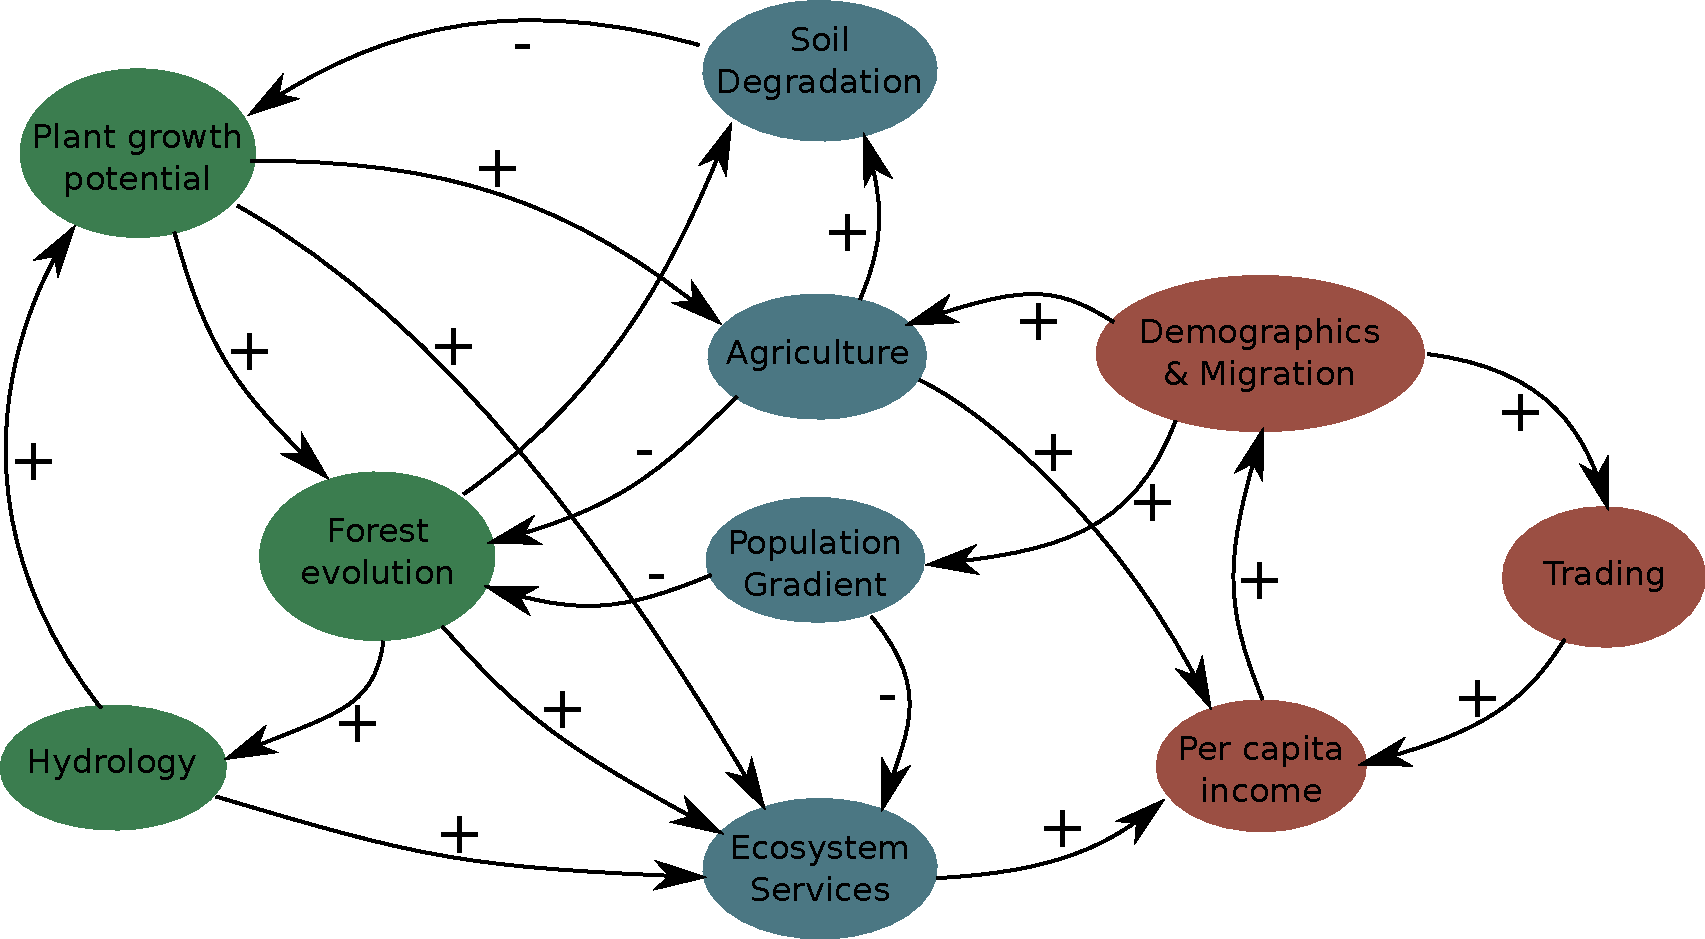
\includegraphics[width=.9 \textwidth]{figures/model_flowchart.pdf}
    \caption{Simplified flowchart of the MayaSim model. Arrows indicate feedbacks between different processes, colors indicate different subsystems namely green for the ecosystem, red for the socio-economic system and blue for processes that interface between the two aforementioned.}
    \label{fig:my_label}
\end{figure}

The MayaSim Model is described in detail by \cite{Heckbert2013}. It represents settlements as agents on a gridded landscape that is used to model the surrounding ecosystem. The ecosystem is described by precipitation, hydrology, agricultural productivity and forest succession, it provides ecosystem services for the Maya population and drives regeneration of soils that have been eroded due to agriculture.

% Ecosystem Processes
\begin{itemize}
    \item \textbf{Precipitation} is driven by empirical data from \cite{Hijmans2005} and varied to mimic paleoclimatic conditions as presented in \cite{Prufer2011}.
    \item \textbf{Hydrology} is modelled by a cellular automata model for surface water flow on the geological elevation profile. For the precipitation on each cell, the water is partly infiltrated and partly moves as water flow along the gradient of surface elevation (also considering the standing water [mm] already at that location) to a neighboring cell. This process is repeated iteratively such that a steady state flow and lake profile forms. 
    \item \textbf{Net primary productivity} is a function of precipitation and temperature as given by the Miamy model in \cite{Lieth1975}.
    \item \textbf{Agricultural productivity} is calculated as with a linear additive model from net primary productivity, soil productivity, surface water flow, and soil degradation.
    \item \textbf{Forest succession} is represented by a cellular automata model where the state of a cell depends on its own history and the state of its neighboring cells. A cell can be in three different states that represent cleared/cropped land, secondary regrowth and climax forest referred to as state 1, 2, and 3 respectively. Forest cells at a small constant rate representing natural disturbance. This rate is linearly amplified by the population density of nearby settlement to represent wood harvesting. The state of a forest cell increases after a certain number of time steps without disturbance to the next higher state where for the increase to state 3 at least three neighboring cells have to be in this state already representing the need to have local vegetation for seed dispersal.
	\item \textbf{Ecosystem Services} are modeled by quantifying the availability of provisioning services of arable soils, fresh water and access to timber as well as food from the forest ecosystem.
\end{itemize}


The socio-economic system of the Maya population is described by settlement nodes with a certain population that generate their per capita income from agriculture, usage of ecosystem services and trading with other settlements. 

% Socio-economic processes
\begin{itemize}
	\item \textbf{Agriculture} drives soil erosion and the clearing of forest where the latter is additionally intensified by the presence of people in the forest using ecosystem services. 
	\item \textbf{Trade} is described by network of trade relations between settlements where settlements above a certain size form trade relationships with their closest neighbors, preferably with those with higher population. Income from trade depends on the total size of the trade network, the possition in the trade network as well as the travel cost to neighboring settlements.
	\item \textbf{Population growth} is described in a simple malthusian fashion with a fixed birth rate and a death rate inversely proportional to per capita income.
	\item \textbf{Migration}: The willingness of people to migrate is driven by low per capita income in existing settlements. If the size of the fraction of the population that exceeds a certain size, it leaves the settlement and tries to establish a new settlement. For the location of their new settlement they sample available locations and maximize their utility depending on available ecosystem services and travel cost depending on distance from the settlement of origin.
\end{itemize}
For detailed description of the above processes, calibration of the model and parameter values please refer to \cite{Heckbert2013} and \cite{Heckbert2013model}

\begin{figure}[!t]
\centering
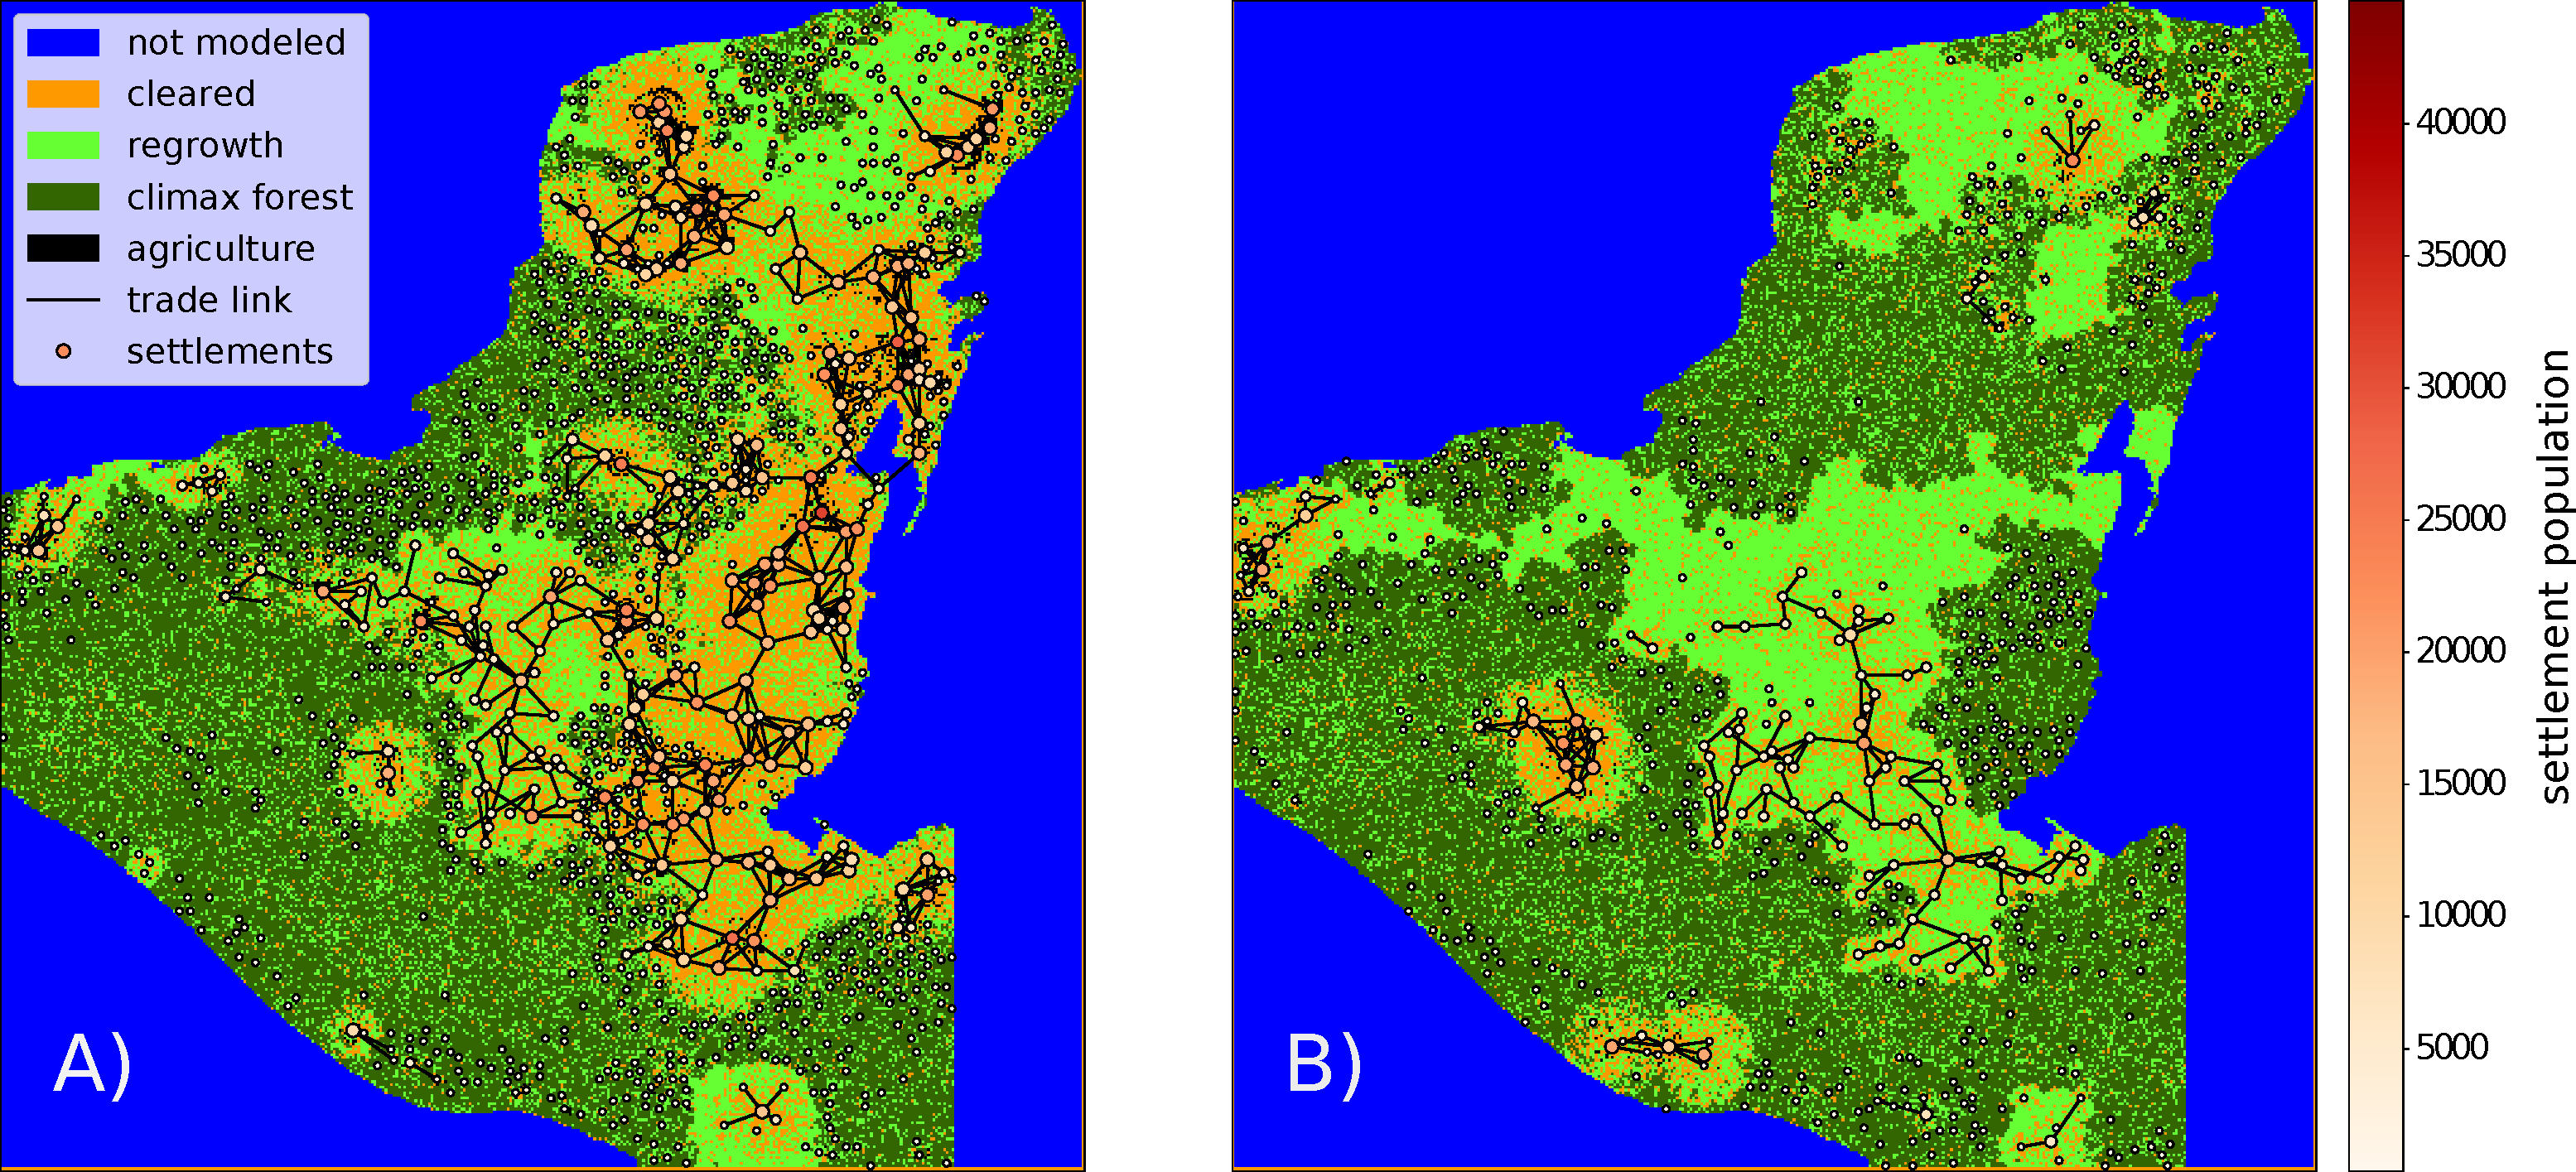
\includegraphics[width=\textwidth]{figures/map_plots.pdf}
\caption{Simulation snapshots showing a complex society in panel A) and a degraded society state in pannel B). Different shades of green indicate different ecosystem states: Black indicates agricultural usage, brown indicates wasteland, light green indicates secondary regrowth, and dark green indicates climax forest. The nodes of the network are settlements with the fill color indicating their population size and the links showing trade relations between them. The brightened area around settlements shows the area that is affected by the settlements usage of ecosystem services. The two different states are taken from the same model run 280 years appart.}
\label{fig:model_snapshot}
\end{figure}

I deviate from the original model in one aspect that I outline and motivate in the following.
In the original model, each settlement needs to use at least one cell for agriculture else it is deleted and its population is assumed to die. I release this constraint as larger settlements are part of a trade network and can trade agricultural produce from other settlements and smaller settlements can get by from income from ecosystem services. I understand that the original version was motivated by the assumption that every settlement must produce some food for its inhabitants, yet this resulted in situations where very large cities rely on the agricultural produce of one cell. Also it neglects the fact that agricultural produce can be traded against products from larger cities' more specialized economies as suggested by \cite{Dahlin2007} as well as the fact that large cities usually had power over smaller settlements in their surroundings and were able to collect tribute from them.

There are some discrepancies between the reference implementation of the model \cite{Heckbert2013model} and the model description paper \cite{Heckbert2013}. In the following processes, our implementation deviates from the reference implementation to be in line with the model description paper: 

\begin{itemize}
    \item In the reference implementation income from agriculture and ecosystem services are calculated as the mean income from cropped cells and cells under a settlements influence respectively. However the model description paper states that income should be calculated as the sum of the yields from cropped cells and cells under the settlements influence. I implemented the process according to the model description paper.
    \item In the reference implementation settlements are not deleted if their population falls below a threshold for subsistence. In our implementation they do.
    \item In the reference implementation settlements build trade relations with their neighboring settlements once their population exceeds a certain threshold. They do however not not lose trade links if their population falls below the respective threshold. In our implementation they do.
\end{itemize}

\section{Methods}
\textit{How can measures of resilience in complex systems be meaningfully applied to geo-simulations?}

% these are the concepts of resilience in complex systems
I use the concept of resilience \citep{Holling1973} aims to describe the response of a system to perturbations and changing environmental conditions. 


As such, it has been defined in two ways: 
first as \emph{engineering resilience} or \emph{persistence resilience} which describes the ability of a system to return to a particular equilibrium or steady-state after a perturbation \citep{Holling1973, Gunderson2000}, and
second, as \emph{transformation resilience} which means ``the capacity of a system to absorb disturbance and reorganize while undergoing change so as to still retain essentially the same function, structure, identity, and feedbacks'' \citep{Walker2004}.

% these concepts have been applied to ecological as well as social-ecological systems
%The concept of resilience has been used abundantly to describe the response of ecological systems to changing environmental conditions due to natural or antropogenic influences \citep{Holling1978, Ludwig1978, Regier1996, Walker1981, Westoby1989, Fiering1982, Walters1986} and more recently also to study SES under the same conditions \citep{Berkes1998, Berkes2003, Adger2000, Adger2005, Galaz2005}

% this is one concept that is used to measure them in social ecological systems
Since the state space of the Mayasim Model is very high dimensional (including the states of each forest cell as well as the positions and state variables of settlements as well as the configuration of the trade network between them), it would be very complicated and tedious to use a persistence resilience approach that measures the response of the full state of the system to changing environmental conditions. Especially because the full state of the model (as we will see later) is not necessarily an equilibrium state but can exhibit endogenous oscillations.
However, one can use a transformation resilience approach to classify the response of the model to exogenous shocks such as drought events.
To do this, one can classify the macroscopic dynamics of the model according to dynamical properties that signal the same function, structure, identity, and feedbacks on the microscopic level of the model. More precisely, in terms of aggregated model variables, one can classify different attractors in the models state space and test whether large perturbations move the model out of the basin of attraction of the desired part of the state space. The simple, one dimensional case of this is illustrated in fig. \ref{fig:basin_stability}.

% this is how I aim to adapt/apply it to geosimulations
Technically, I implement this as follows:
I study the MayaSim model in terms of macroscopic properties and find that it exhibits at least one attractor and one absorbing boundary. The absorbing boundary being zero population from where (due to non existent in-migration into the model space) there is no coming back, the attractor is a complex society state that is subject to a phase transition like event for rising possible income from trade changing from a repeating pattern of development, decline and spatial reorganization to a steady, high population state characterized by a complex trade network between settlements and a degraded ecosystem.

Given these macroscopic dynamical properties of the model, I measure transformation resilience as follows: First I let the system develop until it reaches the complex society attractor. Second, I let the system undergo perturbations of different strength and duration (I reduce the mean annual precipitation for a given percentage over a given period of time). Third, after the perturbation, I measure whether the system returns to the attractor - representing a similar macroscopic state and system functionality with a transformed microscopic configuration - or whether it runs off into the absorbing state with zero population.

Finally, I compare the magnitude of drought events that is sufficient to drive the system into the zero population absorbing state with drought events that can be motivated with empirical data from paleo-climatic records.

\begin{figure}[!t]
\centering
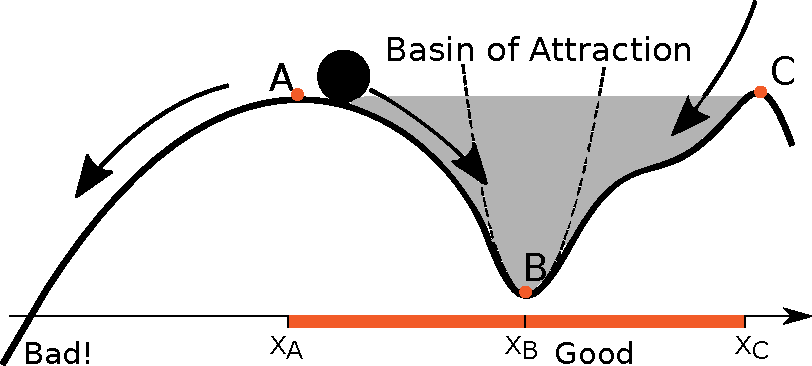
\includegraphics[width=0.5\textwidth]{figures/Basin_Stability.pdf}
\caption{\textbf{Illustration of the concept of resilience/stability}. Imagine a projection of the state space of the system onto a one dimensional manyfold lateral to an attractor or a stable manyfold indicated by B. Then, if the state of the system is in the basin of attraction of B (indicated in grey) its inherent dynamic will eventually return its state back to the stable manyfold. However, if the system is moved sufficiently far away from B (past points A or C) through e.g. a large scale perturbation, it will not return to its previous state, but will move towards an entirely different state space region. Note that for the MayaSim system, this observation holds in terms of macroscopic variables only. After a perturbation, even if the system returns to its previous state in terms of macroscopic variables, its microscopic configuration in terms of geography, demography and ecosystems state can be changed dramatically.}
\label{fig:basin_stability}
\end{figure}

\section{Results}
\begin{figure}[!t]
\centering
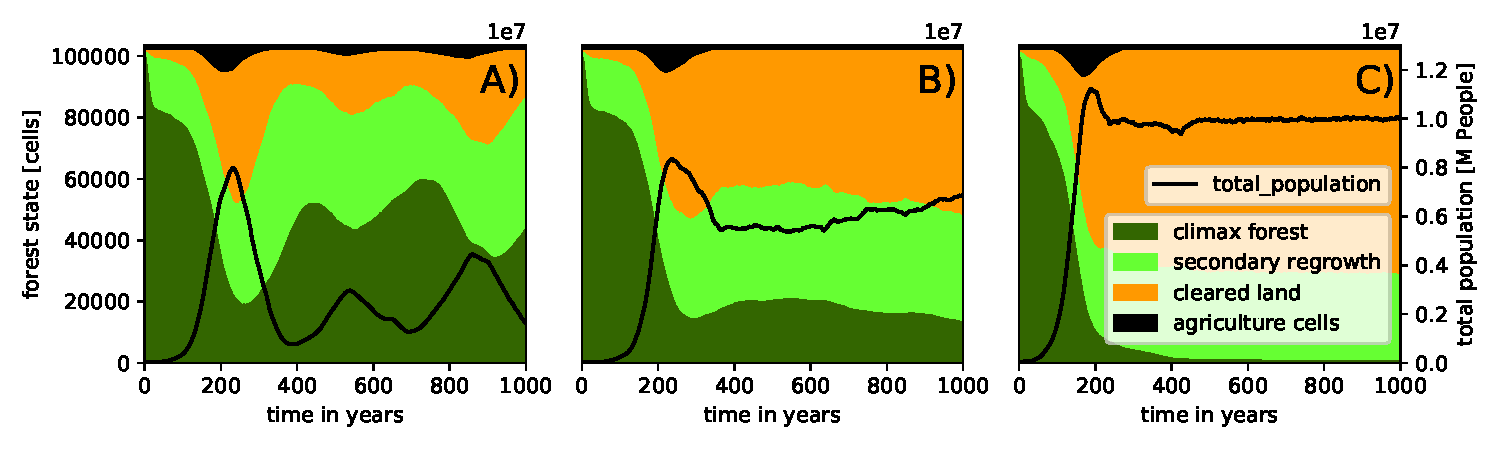
\includegraphics[width=\textwidth]{figures/trajectory.pdf}
\caption{Example trajectories of simulation runs with different possible income from trade relations $r_{trade}$. Possible income from trade relations increases from A: $r_{trade}=6000$, B: $r_{trade}=7000$ to C: $r_{trade}=8000$. The colored stack plot shows the fraction of land in different states on the left axis. The black line shows the total population on the right axis.}
\label{fig:trajectory}
\end{figure}

\subsection{Bifurcation Analysis}
%\textit{Is the overshoot and collapse reported with the original model inherent or rather a result of parameter choices and selection of the time window?}
% Motivate the variation of $r_{trade}$ and $r_{es}$.

Income per capita is the main driver of population growth in the Mayasim model. Income is calculated as a linear combination of three different sources of income: agriculture, ecosystem services and trade. The parametrization of income from agriculture can be sensibly done as e.g. in \cite{ertsen2018}. However, the parameters for income from trade $r_{trade}$ and ecosystem services $r_{es}$ are more difficult to calibrate. Therefore, I analyze their influence in more detail in the following.

% Discuss the trajectories for different values of r_trade

Results from model runs with different choices of $r_{trade}$ are shown in figure \ref{fig:trajectory}. For different choices of the possible income from trade, the model exhibits fundamentally different dynamics:
\begin{itemize}
  \item In fig. \ref{fig:trajectory} A the total population and the aggregate number of climax fores cells exhibit a predator prey like dynamic that can be explained as follows: Climax forest results in soil regeneration as well as a high level of ecosystem services which drives per capita income and thereby population growth. Growing population on the other hand leads to disruption of the fores ecosystem resulting in its degeneration as well as extensive agriculture, that benefits from regenerated soils but also drives clearing of forest and soil degeneration.
  \item In fig. \ref{fig:trajectory} B higher possible income from trade leads to the onset of the decoupling of population dynamics from the state of the surrounding ecosystem. 
  \item In fig. \ref{fig:trajectory} C the society, once in its complex state characterized by strong trading relations, is no longer dependent on the state of the surrounding ecosystem.
  \item A closer look at the results in fig. \ref{fig:trajectory} A also shows that they are not just a result of a simple predator prey dynamic but rather represent a pattern of of regionally increasing complexity, collapse and restructuring not unlike what the archeological record from the area suggests.
\end{itemize}
These results also suggest, that the initial overshoot and collapse dynamics presented in \cite{Heckbert2013} may have been only part of the picture. The results suggest that the pronounced overshoot and collapse is at least partially caused by the initial conditions that combine a perfectly intact ecosystem with a small initial population that, given the modeling choices is implicitly assumed to have full knowledge of agricultural techniques, trade and ecosystem usage. They show, that after the initial overshoot and collapse a more balanced feedback between human settlements and the surrounding ecosystem is possible as displayed in \ref{fig:trajectory} A.

\begin{figure}[!t]
\centering
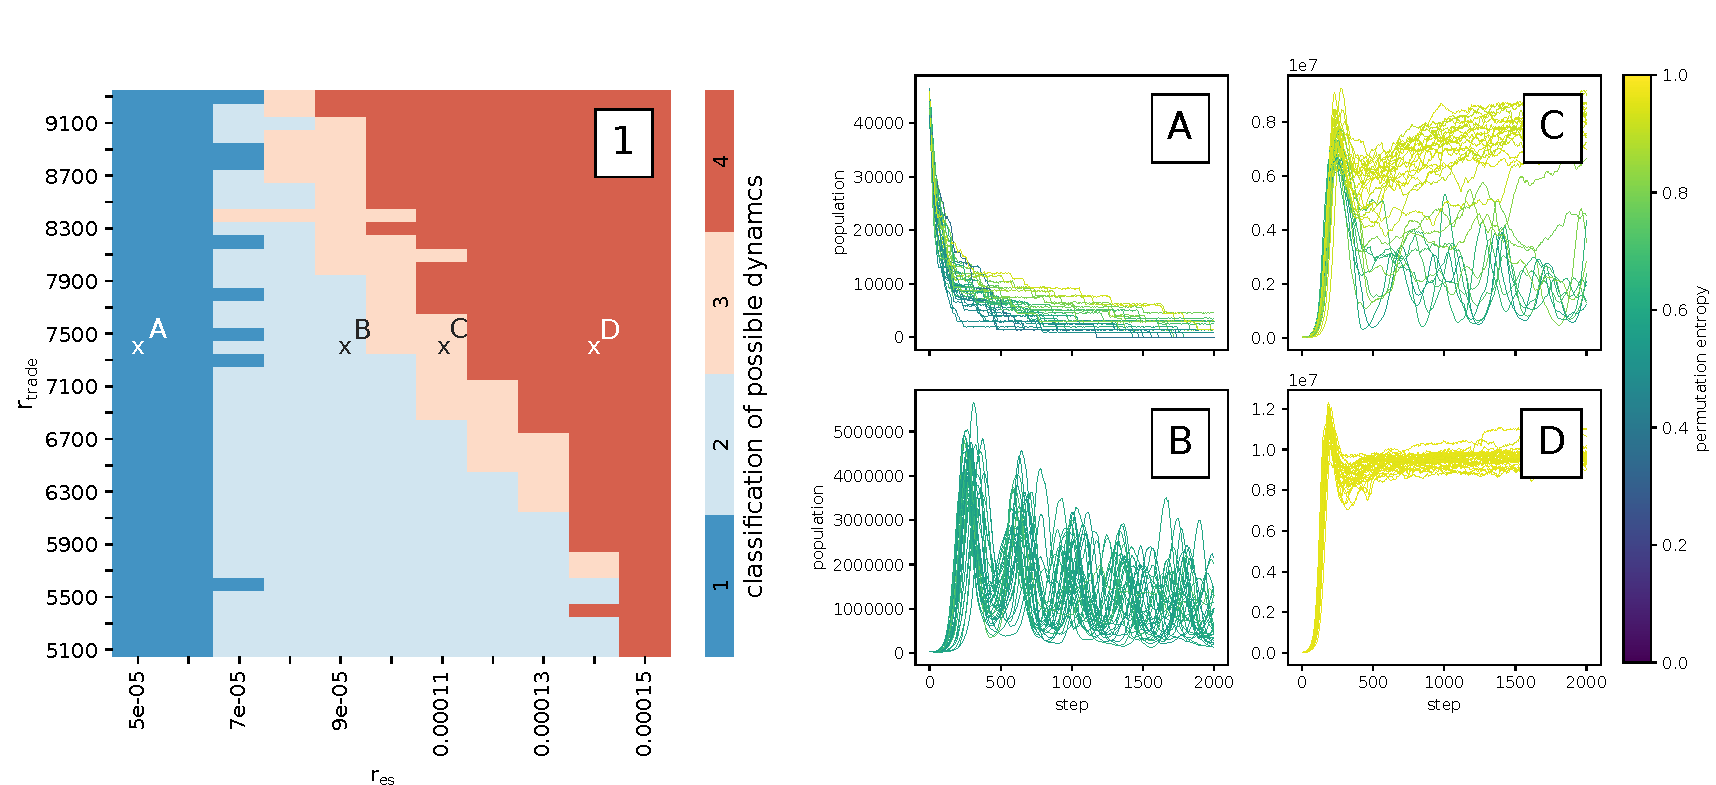
\includegraphics[width=\textwidth]{figures/classified_dynamics.pdf}
\caption{\textbf{Classification of model dynamics for different values of income from trade relations and ecosystem services.} Results are calculated from an ensemble of 30 runs for each combination of parameter values. For each of these 30 runs, I calculate the permutation entropy of the trajectory for $t>500$ i.e. after the initial overshoot and collapse. I show sets of trajectories for different parameter values in panels A, B, C and D. The color of the trajectories indicates their permutation entropy. The specific parameter values are marked in panel 1. From the distribution of the permutation entropy of these ensembles of trajectories, I classify the dynamic regime of the model given in panel 1. Regime 1 indicates the monotonous decline in population as in panel A, regime 2 indicates oscillatory behavior of the population as in panel B, regime 4 indicates a stable high population state as in panel D and regime 3 indicates the coexistence of the two aforementioned dynamics as in panel C.}
\label{fig:permutation_entropy}
\end{figure}

% Discussion of different possible dynamic regimes / bifurcation analysis

To systematically expand on this finding, I generated model trajectories for a wide range of values
for the possible income from trade relations and the possible income from ecosystem services in the model and classified the resulting trajectories with regards to their dynamical properties. A suitable measure for this task is permutation entropy as introduced by \cite{Bandt2002}. This measure classifies trajectories by interpreting them as a series of ordinal patterns of a predefined length and then calculating the entropy of the distribution of said patterns. This entropy is normalized between zero and one. To give some points of reference: For a constant trajectory, this results in a permutation entropy of zero. For a sine wave, this results in a value of one half and for uniformly distributed noise, this results in a value of one.

The classification of the dynamical properties of the model for different parameter values is given in fig. \ref{fig:permutation_entropy} 1. It shows that the model exhibits a bifurcation like behavior where depending on the parameter values different qualitative behaviors are possible. First, a slow decline in population that eventually leads to extinction as displayed in fig. \ref{fig:permutation_entropy} A, second, an oscillatory with a predator prey like dynamic between the Maya population and the forest ecosystem fig. \ref{fig:permutation_entropy} and also fig. \ref{fig:trajectory} A, third, a stable state with high population that is primarily supported by income that is generated from trade as in fig. \ref{fig:permutation_entropy} D and fig. \ref{fig:trajectory} C and fourth, a region where oscillatory behavior and stable high population states can coexist as in fig. \ref{fig:permutation_entropy} C.

% Discussion of stable high population regime that is primarily supported by trade income

Particularly the stable high population state deserves a closer look. As fig. \ref{fig:trajectory} C shows, this state is characterized by low agricultural activity and a degraded ecosystem such that income from trade is the primary source of income. Even though the particulars of trade theory are controversial among economists, there is consensus in that increase in welfare through trade originates in either better division of labor or exchange of locally different input factor endowments. This means, that income from trade without other sources of economic productivity is not a realistic scenario. This sheds light on the limits of the trade model that is used in the MayaSim Model where income from trade is generated through the establishment and maintenance of a trade network amongst sufficiently large settlements i.e. through societal complexity alone. This is a plausible approximation as long as there are substantial sources of income other then trade but becomes unrealistic as soon as trade becomes the primary source of income and even more, once income from trade stabilizes the high population levels that are necessary to sustain the trade relations that generated said trade income to begin with.

Therefore, I conclude that the stable high population attractor is a pathological consequence of the approximate implementation of trade in the model and can be discarded for considerations about the archeological realities of the ancient Maya.
Consequently, for the following analysis of system resilience with respect to drought events, I use parameters that lead to oscillatory behavior where income from trade relations can be considered realistic.

% Discussion of results from drought events.

\begin{figure}[ht]
\centering
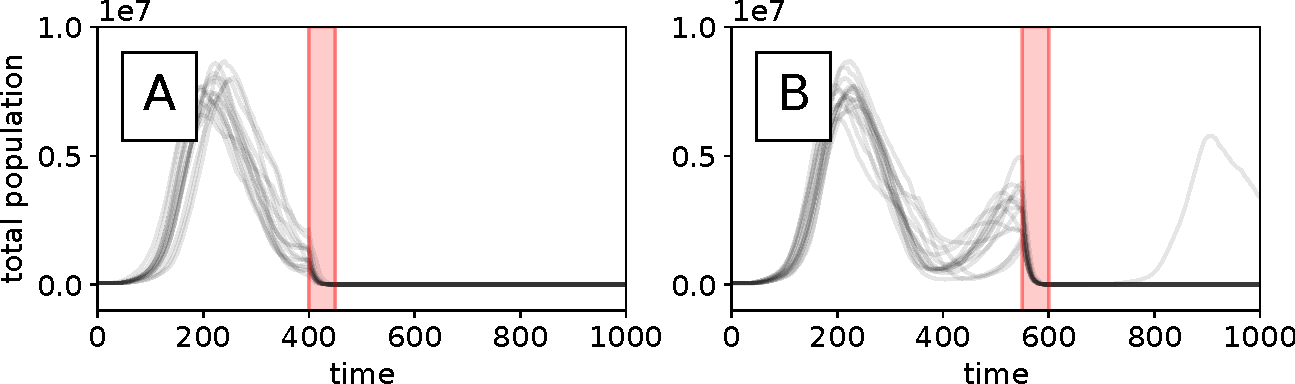
\includegraphics[width=\textwidth]{figures/population_with_drought.pdf}\vspace{.3 cm}
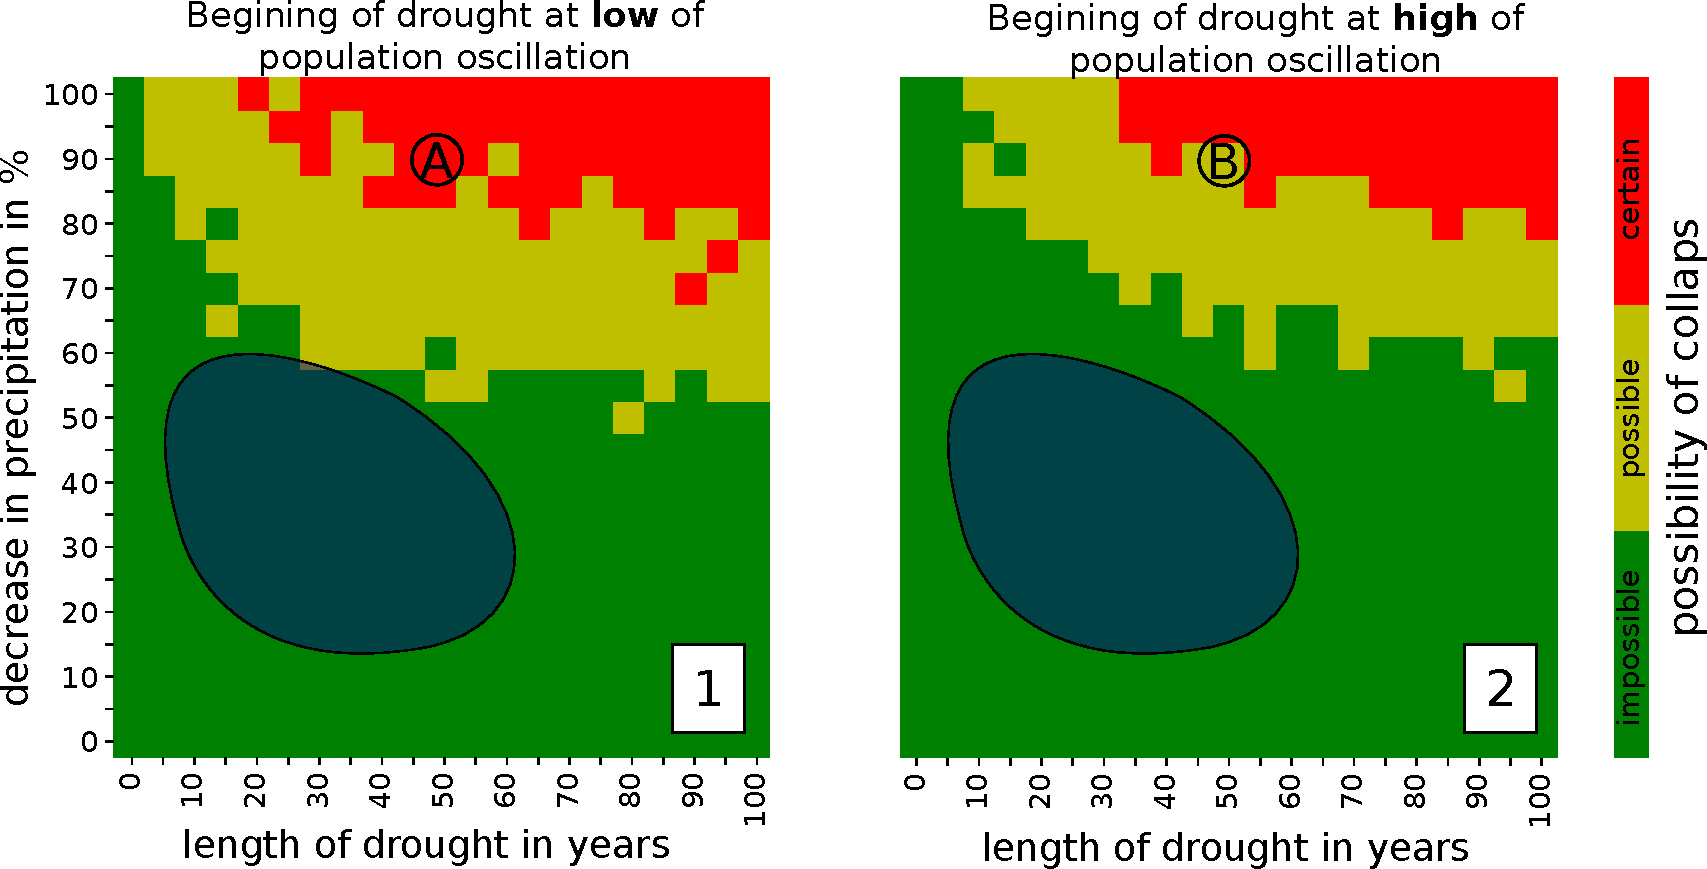
\includegraphics[width=\textwidth]{figures/possibility_of_collapse.pdf}
\caption{\textbf{Measurement of Transformation-Resilience with respect to drought events of different length, severity and timing compared to estimates from paleo-climatic data.} Results are calculated from an ensemble of 15 simulation runs for each combination of drought length and severity. Panels 1 and 2 differ with respect to the timing of drought events. In panel 1 the beginning of the reduction of precipitation starts approximately at the bottom of the oscillations of total population whereas in panel 2 it starts at its top. To illustrate this, panels A and B show individual trajectories of the total Maya population for drought events of the same length and severity but with different timing. Parameter values for length and severity of drought events in panels A and B are also marked in panels 1 and 2 respectively.
I classify resilience in terms of the possibility of collapse i.e. extinction of the human population for drought events of different length, severity and timing.
Technically, this means that I disregard the systems micro state and only estimate the probability for for a drought event to force the social ecological system out of the basin of attraction of its habitable attractor and then classify the parameter space of length and severity of drought events in regions where this probability is either zero, one or in between. These regions are marked in green, yellow and red respectively in panels A and B. The region of parameter values for length and severity of drought events that can be motivated by evidence from paleo-climatic records is marked in blue in panels 1 and 2.}
\label{fig:stability_analysis}
\end{figure}

\subsection{Drought Resilience}
\textit{Can a drought event be responsible for the terminal decline of the Maya civilization on the Yucatan peninsula, given the assumptions of the model?}

As discussed in the methods section, the ability of the system to recover after a large scale disturbance to a state that is macroscopically equivalent to that before the disturbance -- regardless of their microscopic configuration -- can be seen as a measure of resilience with respect to said disturbance.

To better understand the possibility of a large drought event leading to a lasting change in the Mayan population on the Yucatan peninsula, I analyse the models resilience to such drought events of different length, severity and timing. The results in fig. \ref{fig:stability_analysis}, panel A and B show the trajectories of total population for different model runs with equal model parameters but different timing of drought events. In panel A a drought event with length of 50 time steps and precipitation reduction of 90\% starts as the oscillation of population levels is a low. This leads to the complete disappearance of the Maya population in all simulated cases. A drought event of the same magnitude but beginning at the peak of the oscillation as in panel B also results in a severe reduction in population over the time of the drought event. However, if a small population survives, it is able to recover and to reach population levels comparable to those before the drought event.

To analyze the impact of drought events systematically, I show results for drought events with timing like in panels A and B but for different length and severity in panels 1 and 2. To abstract from the presentation in terms of trajectories, I classify the results of an ensemble of model runs for each set of parameter values in the following way: If in all model runs, the Maya population vanishes, I say that collapse is certain and mark the parameter combination red. If this happens only in some of the model runs, I say that collapse is possible and mark the parameter combination in yellow and if the Maya population vanishes in none of the simulation runs, I say that collapse is impossible and mark the parameter combination in green.

These results show, that the timing of drought events does have the effect on the measured resilience that can also be expected. A drought of the same length and severity can have a more dire effect if it hits at the moment when population levels are already low.

This abstract representation of the impact of drought events enables us to draw a comparison with the paleo-climatic evidence available:
\cite{Stahle2011} find evidence for drought of 25y duration but make no estimate for precipitation reduction.
\cite{Evans2018} estimate a reduction in annual precipitation of 41\%-52\% with up to 70\% during peak drought but no make specification as to the length of drought events.
\cite{Medina-Elizalde2010} find evidence for six droughts between C.E. 800 and 909 with a maximum reduction in annual precipition of ~52\% and a maximum length of 18 years.
\cite{Medina-Elizalde2012} estimate a reduction in annual precipitation of 25\% to 40\% over more than 14 years.
\cite{Kennett2012} mention a -40\% reduction in annual precipitation between 820 and 870 C.E. as well as a 100 year drought starting in 1020 C.E.


Overall the different estimates for historic drought events reach from a reduction of annual precipitation of 25\% to 52\% over an extended period of 25 up to 50 years. I mark this region in blue in fig. \ref{fig:stability_analysis} panel 1 and 2 for comparison.

This comparison shows, that even with unfortunate timing of drought events, the values for length and severity of drought events that can be motivated from paleo-climatic records has quasi zero intersection with the parameter values that possibly lead to extinction of the Maya population in our model.

I conclude, that given the economic and behavioral assumption about the Maya civilization that are the basis of the MayaSim model, drought events alone are a very unlikely cause for a long lasting severe impact on the Maya civilization on the Yucatan peninsula.

\section{Discussion and Conclusion}

% Short recap of paper
This paper reimplements and improves upon an established/existing agent-based geosimulation model for the ancient Maya civilization on the Yucatan peninsula.
I analyze the model with respect to sensitivity to key parameters and find that is capable of a richer dynamic variety than presented in the original studies.
I also analyze the resilience of the model dynamics with respect to drought events compare the results with data from paleoclimatic records.

% comparison of our model dynamics to Heckberths original results
The origininal study \citep{Heckbert2013} and reference implementation \citep{Heckbert2013model} of the MayaSim model presents an overshoot and collapse pattern of the ancient Maya civilisation and attributes the cause of the collapse to changing climatic conditions, specifically decreasing annual precipitation in the region. After a close examination of the reference implementation and comparing its results with the results of our improved implementation with come to a different conclusion. I rather propose to attribute the pronounced overshoot and collapse pattern of the original model to two particular modelling choices in combination with the models initial conditions. Namely the fact that in the original implementation settlements were deleted if and only if they abandon their last agriculture cell in combination with the choice to model income from agriculture and ecosystem services as the mean rather than the sum of income from cells that are used for ecosystem services and agriculture respectively. This means that even a large settlement can survive on the income from one cell of agriculture only to suddenly vanish, once this last patch of agriculture becomes uneconomic. On an aggregated level this means that the feedback from the deteriorating ecosystem due to deforestation and soil erosion impacts the settlement infrastructure delayed but then suddenly all the more forceful. In combination with the initial condition of a small population in a fully intact ecosystem that can quickly expand without feeling the effects of its unsustainable growth this strongly supports the observed pattern.

In our updated model, I chose to model these two processes differently and as I believe more credibly. I model income from agriculture and ecosystem services as the sum of income that is generated from individual cells that are under a settlements influence and I model the abandonment of settlements such that they are deleted once their population drops under a minimum threshold that is necessary for subsistence.

This means that the effect of the deterioration of the surrounding ecosystem impacts the affected settlements directly and without delay. Consequently, the initial overshoot is less pronounced in our adaptation of the model. However, I also find that following the initial overshoot this adaptation produces a pattern of development, climax, deterioration and spatial reorganization of regional centers in close interdependence with the surrounding ecosystem that much resembles the archeologic record. I find that this oscillating dynamic strongly depends on the parameterization of the model and that for variation of key parameters the model undergoes two transitions. The first transition leads from a state where the initial population continuously deteriorates to eventually vanish to the previously described state of cyclical rise and fall of regional centers. The second transition leads from this state of cyclical dynamics to another state of stable, self sustaining high population in a deteriorated ecosystem. Of these, only parametrizations that lead to cyclical behavior of the model can be considered realistic.

% discussion of results from analysis of model resilience w.r.t. drought events
Subsequently, I test the resilience of the updated model with a realistic parameter setting with respect to drought events of different severity, duration and timing. In this study I find that even for drought events that even drought events that reduce the mean annual precipitation to half for a duration of 50 hears do not lead to the extinction of the Maya population in the model. This holds true even if the drought event hits the population in a state where it is deteriorized to begin with due to its inherent dynamics. Comparing these results with the length and severity of drought events that can be motivated from historical records, I find that none of them would be sufficient to eventually break up the Maya civilization in the model.
From this I conclude that given the assumption that the model is grounded on, climate variability as single cause of the deterioration of the ancient Maya civilization can be ruled out. Rather this supports the argument that in addition to climate variability other factors had to play a role in the fundamental transformation of the Maya society during the Terminal Classic Period \citep{Masson2012}. Others have also already argued that in only internal societal changes could have caused this transformation under the conditions of increased aridity and overly stressed ecosystems \citep{Turner2012a}.

% discuss how models could better picture societal change on an individual level
One way to address this this problem from a modeling perspective would be to separate judgement from actions in the modeling of individual (human) agents. Possible actions are usually confined to a finite set that is limited by the conditions of the agents environments but judgements can evolve more freely as a way to  allow agents to change. Technically, this can be implemented e.g., with techniques from reinforcement learning \citep{Bu2008} or by implementing different heuristic decision models. Such heuristic decision models allow for an adaptive mental model of individual agents in terms of simple algorithmic rules that they use to integrate the information from their environment to select one of different possible actions.
This would allow for agents to adapt to changing circumstances in their modeling environment. While modeling paradigm does not change the fundamental fact that agents in a model cannot have anything resembling free will, it would nevertheless allow for models to depict changes in societal structure that are grounded in individually changing perceptions of reality.

